 % !TEX root = article.tex

\section{Experimental Evaluation}
\label{se:experiments}

In this section we present a preliminar experimental study of our OSR technique in TinyVM, a proof-of-concept virtual machine based on LLVM's JIT compiler MCJIT. TinyVM supports interactive invocations of functions and it can compile LLVM IR either generated at run-time or loaded from disk. The main design goal behind TinyVM is the creation of an interactive environment for IR manipulation and JIT-compilation of functions: for instance, it allows the user to insert OSR points in loaded functions, run optimization passes on them or display their CFGs, repeatedly invoke a function for a specified amount of times and so on. TinyVM supports dynamic library loading and linking, and comes with a helper component for MCJIT that simplifies tasks such as handling multiple IR modules, symbol resolution in presence of multiple versions of a function, and tracking native code and other machine-level generated object such as Stackmaps.

TinyVM is thus an ideal playground to exercise our OSR technique, and we use it to run performance measurements on the shootout test suite, also known as the Computer Language Benchmark Game~\cite{shootout}. The list of benchmarks and their description is reported in Table~\ref{tab:shootout}; four of them - namely {\tt b-trees}, {\tt mbrot}, {\tt n-body} and {\tt sp-norm} - are evaluated against two workloads of different size.

\begin{table} 
\begin{center}
\begin{small}
    \begin{tabular}{ |c|c| }
        \hline
        {\em Benchmark} & {\em Description} \\ 
        \hline
        \hline
        b-trees & Adaptation of a GC bench for binary trees \\ 
        \hline
        fannkuch & Fannkuch benchmark on permutations \\ 
        \hline
        fasta & Generation of DNA sequences \\ 
        \hline
        fasta-redux & Generation of DNA sequences (with lookup table) \\ 
        \hline
        mbrot & Mandelbrot set generation \\ 
        \hline
        n-body & N-body simulation of Jovian planets \\ 
        \hline
        rev-comp & Reverse-complement of DNA sequences \\ 
        \hline
        sp-norm & Eigenvalue calculation with power method \\ 
        \hline
    \end{tabular} 
\end{small}
\end{center}
\caption{\label{tab:shootout} Description of the shootout benchmarks} 
\end{table}

\subsection{Setup}

We generated the IR modules for our experiments with clang, starting from the C version of the shootout suite. In the version of the code we will refer to as {\em unoptimized}, no LLVM optimization passes were performed on the code other than {\em mem2reg}, which promotes memory references to register references and constructs the SSA (Static Single Assignment) form. Starting from this version, we then generate an {\em optimized} version performing using the LLVM IR optimizer {\tt opt} at {\tt -O1} optimization level.

Experiments were performed on an octa-core 2.3 Ghz Intel Xeon E5-4610 v2 with 256+256KB of L1 cache, 2MB of L2 cache, 16MB of shared L3 cache and 128 GB of DDR3 main memory, running Debian Wheezy 7, Linux kernel 3.2.0, LLVM 3.6.2 (Release build, compiled using gcc 4.7.2), 64 bit.

For each benchmark we performed 10 trials preceded by an initial warm-up iteration; reported confidence intervals are stated at 95\% confidence level.

\subsection{Results}

\begin{itemize}
\item {\bf Message 1}: how much does a never-firing OSR point impact code quality? We run a program with one or more OSR points, and we measure the slowdown given by factors such as cache effects (due to code bloat), register pressure, etc. due to the presence of the OSR points.
\item {\bf Message 2}: what is the overhead of an OSR transition to the same function? We run a program with a controlled OSR transition, e.g., with a counter that fires the OSR. Here we measure the impact of the actual OSR call. We compute for each benchmark: 1) the average time per OSR transition; 2) the number of transferred live variables; 3) the total benchmark time with an always-firing OSR at each iteration of the hottest loop; 4) the total benchmark time with a never-firing OSR at each iteration of the hottest loop (baseline); 5) the number of iterations of the hottest loop (equals the number of OSR transitions).
\item {\bf Message 3}: what is the overhead of the library for inserting OSR points? We compute for each benchmark: 1) time required by insertOpenOSR (OSR point insertion + creates stub); 2) time required by insertFinalizedOSR (OSR point insertion + generation of continuation function); 3) time required for generating continuation function.
\end{itemize}

\paragraph{Impact on code quality}
In order to measure how much a never-firing OSR point might impact code quality, we analyzed the source-code structure of each benchmark and profiled its run-time behavior to identify performance-critical sections for OSR point insertion.

For iterative benchmarks, we insert an OSR point in the body of their hottest loops. We classify a loop as hottest when its body is executed for a very high cumulative number of iterations (e.g., from a few thousands up to billions) and it either calls the method with the highest {\em self} time in the program, or it performs the most computational-intensive operations for the program in its own body. These loops are natural candidates for OSR point insertion, as they can be used - as in the Jikes RVM - to enable more dynamic inlining opportunities, with the benefits from several control-flow (e.g., dead code elimination) and data-flow (e.g., constant propagation) optimizations based on the run-time values of the live variables. In the shootout benchmarks, the number of such loops is typically 1 (2 for {\tt spectral-norm}).

For {\tt b-trees} - the only benchmark in our suite showing a recursive pattern - we insert an OSR point in the body of the method that accounts for the largest {\em self} execution time of the program. Such an OSR point might be useful to trigger recompilation of the code at a higher degree of optimization, or to enable some form of dynamic optimization (for instance, in a recursive search algorithm we might want to inline the comparator method provided by the user at the call).

Results for the unoptimized and optimized versions of the benchmarks are reported in Figure~\ref{fig:code-quality-base} and \ref{fig:code-quality-O1}, respectively. For both scenarios we observe that the overhead is very small, i.e. less than $1\%$ for most benchmarks and less than $2\%$ in the worst case. In some cases, code might run slightly faster after OSR point have been inserted due to cache and instruction alignment effects. We analyzed the code produced by the x86_64 back-end: the OSR machinery is lowered into three native instructions that load a counter in a register, compare it against a constant value and jump to the OSR block accordingly. The number of times the OSR condition is checked for each benchmark is the same as in the experiments reported in Table~\ref{tab:sameFun}.
  
\paragraph{Overhead of OSR transitions}

Table~\ref{tab:sameFun} reports for each benchmark an estimate of the average cost of performing an OSR transition to a function identical to the running one. For each benchmark we compute the difference in terms of total CPU time when an always-firing or a never-firing OSR point is inserted in the code, respectively; we then normalize this difference against the number of fired OSR transitions.

Hot code portions for OSR point insertion are picked as in the experiments for code quality. However, as our goal for hot loops is to perform an OSR transition at each iteration, inserting an always-firing OSR point in the enclosing function is not an option, because the function we OSR into should then fire an OSR itself, leading eventually to a very large number of active stack frames. Depending on [...]

\begin{table*} 
\begin{center}
\begin{small}
    \begin{tabular}{ |c|c|c|c|c|c|c|c| }
        \cline{3-8}
        \multicolumn{2}{c|}{} & \multicolumn{3}{c|}{Base version} & \multicolumn{3}{c|}{Optimized code} \\
        \hline
        Benchmark & Fired OSR transitions & Live values & Avg time (ns) & Overhead (\%) & Live values & Avg time (ns) & Overhead (\%) \\ 
        \hline
        \hline
        b-trees & 605\,377\,887 & 2 & 1.731 & 3.96 & 3 & 0.974 & 2.29 \\ 
        \hline
        b-trees-large & 2\,689\,946\,975 & 2 & 1.749 & 3.90 & 3 & 1.423 & 3.30 \\ 
        \hline
        fannkuch & 399\,168\,000 & 0 & 1.793 & 1.73 & 0 & 0.621 & 0.59 \\ 
        \hline
        fasta & 400\,000\,000 & 2 & 2.335 & 7.39 & 2 & 2.699 & 8.23 \\ 
        \hline
        fasta-redux & 400\,000\,000 & 4 & 2.306 & 20.13 & 4 & 2.269 & 19.69 \\ 
        \hline
        mbrot & 256\,000\,000 & 15 & 5.016 & 2.40 & 15 & 3.628 & 1.75 \\ 
        \hline
        mbrot-large & 1\,024\,000\,000 & 15 & 5.268 & 2.53 & 15 & 4.637 & 2.25 \\ 
        \hline
        n-body & 50\,000\,000 & 3 & 2.952 & 1.65 & 3 & 6.929 & 3.59 \\ 
        \hline
        n-body-large & 500\,000\,000 & 3 & 2.953 & 1.64 & 3 & 6.953 & 3.60 \\ 
        \hline
        rev-comp & 6\,172\,843 & 8 & -10.158 & -1.10 & 8 & 8.267 & 0.92 \\ 
        \hline
        sp-norm & 1\,210\,000\,000 & 2 & 0.772 & 14.76 & 2 & -0.030 & -0.57 \\ 
        \hline 
        sp-norm-large & 19\,360\,000\,000 & 2 & 0.778 & 14.89 & 2 & -0.003 & -0.07 \\
        \hline
    \end{tabular} 
\end{small}
\end{center}
\caption{\label{tab:sameFun}Average cost of an OSR transition to the same function.} 
\end{table*}

% figure
\ifdefined\noauthorea
\begin{figure}[t]
\begin{center}
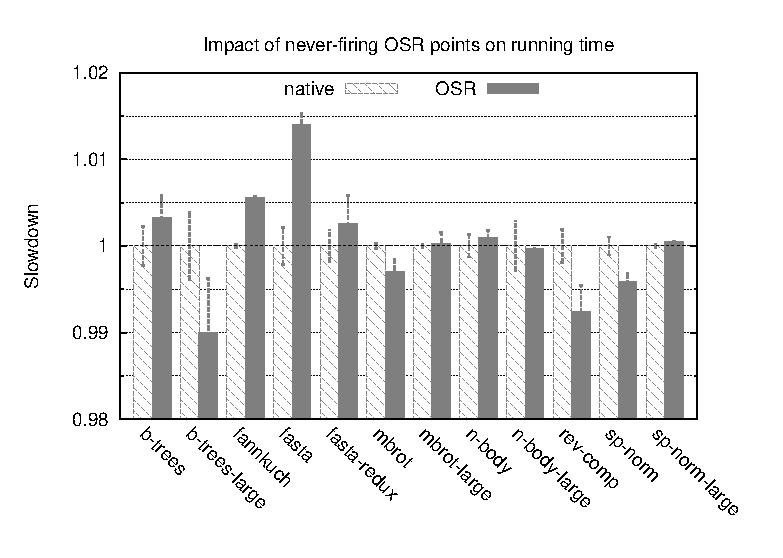
\includegraphics[width=0.95\columnwidth]{figures/code-quality-noBB/code-quality-noBB.eps}
\caption{\label{fig:code-quality-base} \protect\label{fig:code-quality} Impact on running time of never-firing OSR points inserted inside hot code portions (unoptimized code).
  
  
  }
\end{center}
\end{figure}
\fi

\ifdefined\noauthorea
\begin{figure}[t]
\begin{center}
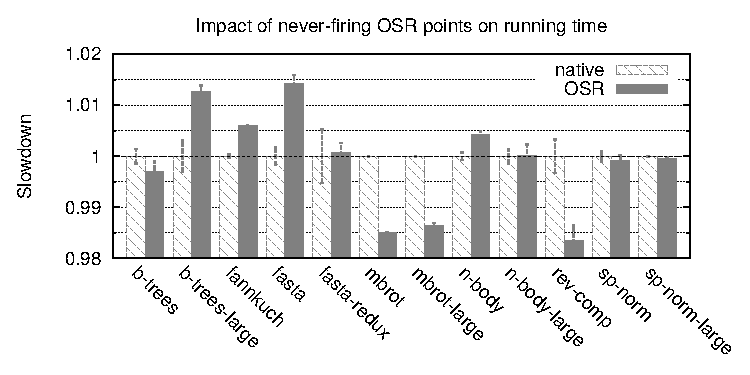
\includegraphics[width=0.95\columnwidth]{figures/code-quality-O1-noBB/code-quality-O1-noBB.eps}
\caption{\label{fig:code-quality-O1} \protect\label{fig:code-quality-O1} Impact on running time of never-firing OSR points inserted inside hot code portions (optimized code).
  
  
  
}
\end{center}
\end{figure}
\fi

\ifauthorea{\newline}{}
\paragraph{OSR machinery insertion}
[...]

\begin{table} 
    \begin{tabular}{ |c|c|c|c|c|c|c|c|c| }
        \cline{3-9}
        \multicolumn{2}{l|}{} & \multicolumn{3}{c|}{open OSR} & \multicolumn{4}{c|}{resolved OSR} \\ 
        \cline{3-9}
        \multicolumn{2}{l|}{} & point & stub & IR code & point & \multicolumn{2}{|c|}{OSRDest generation} & IR code \\ 
        \cline{1-2} \cline{7-8}
        benchmark & IR instructions & insertion & generation & verification & insertion & total & avg per inst & verification \\ 
        \hline
         &  &  &  &  &  &  &  &  \\ 
        b-trees & 13 & 15.40 & 28.32 & 58.03 & 14.31 & 76.13 & 5.86 & 65.15 \\
        \hline
        fannkuch & 50 & 14.16 & 18.66 & 86.77 & 12.84 & 208.03 & 4.16 & 98.98 \\
        \hline
        fasta & 38 & 12.93 & 27.07 & 76.84 & 13.01 & 250.39 & 6.59 & 98.08 \\
        \hline
        fasta-redux & 55 & 13.79 & 23.44 & 72.90 & 9.32 & 258.36 & 4.70 & 105.76 \\
        \hline
        mbrot & 77 & 15.96 & 27.39 & 79.88 & 15.30 & 384.61 & 4.99 & 103.72 \\
        \hline
        n-body & 19 & 14.31 & 19.73 & 76.76 & 11.58 & 88.73 & 4.67 & 83.84  \\
        \hline
        rev-comp & 145 & 16.31 & 39.99 & 132.87 & 13.90 & 810.84 & 5.59 & 201.40 \\
        \hline
        sp-norm & 28 & 15.31 & 27.50 & 68.32 & 12.41 & 154.54 & 5.52 & 75.34 \\ 
        \hline
    \end{tabular} 
\caption{\label{tab:instrTime} OSR machinery insertion in optimized code. Time measurements are expressed in microseconds.} 
\end{table}
  

  
  
  
  
  
  
  
  
  
  
  
  
  
  
  
  
  
  
  
  
  
  
  
  